\documentclass[a4paper,12pt]{extarticle}
\usepackage[table,xcdraw]{xcolor}
\usepackage{pgfplots}
\usepackage[unicode, pdftex]{hyperref}
\usepackage[T2A]{fontenc}
\usepackage[utf8]{inputenc}
\usepackage[english,russian]{babel}
\usepackage{amsmath,amsfonts,amsthm, mathtools}
\usepackage{amssymb}
\usepackage{graphicx}
\graphicspath{{images/}}
\usepackage{wrapfig}
\usepackage{floatrow}
\usepackage{setspace}
\usepackage[headings]{fancyhdr}
\usepackage[margin=10pt,font={small,stretch=0,9},labelfont=bf,labelsep=period,
justification=centerlast]{caption}
\usepackage{array,tabularx,tabulary,booktabs}
\RequirePackage{multirow}
\RequirePackage{multicol}
\RequirePackage{longtable}
\usepackage{indentfirst}
\usepackage{hyperref}
\usepackage{icomma}
\newcommand*{\hm}[1]{#1\nobreak\discretionary{}
	{\hbox{$\mathsurround=0pt #1$}}{}}
\usepackage{soulutf8} 
\usepackage{etoolbox} 
\usepackage{geometry}
\geometry{top=20mm}
\geometry{bottom=20mm}
\geometry{left=20mm}
\geometry{right=20mm}
\DeclareMathOperator{\sgn}{\mathop{sgn}}
\usepackage[OT1]{fontenc}
\usepackage{amsmath}
\usepackage{amsfonts}
\usepackage{amssymb}
\usepackage{wasysym}
\usepackage{wrapfig}
\usepackage{physics}
\usepackage[normalem]{ulem}
\graphicspath{{pictures/}}
\DeclareGraphicsExtensions{.png,.jpg,.jpeg}
\usepackage{indentfirst}
\usepackage[T2A]{fontenc}
\usepackage{subfigure}
\usepackage{fancyhdr}
\usepackage{caption}

\usepackage{tabularx}
\usepackage{floatrow}
\usepackage{multicol}
\usepackage{lastpage}

\pgfplotsset{
  MyStyle1/.style={
    axis lines = middle,
    enlargelimits = true,
    grid=both,
    grid style={line width=.1pt, draw=gray!10},
    major grid style={line width=.2pt,draw=gray!50},
    minor tick num=5,
    enlargelimits=0.05,
    ticklabel style={font=\tiny,fill=white},
    xlabel style={at={(ticklabel* cs:1)},anchor=north west},
    ylabel style={at={(ticklabel* cs:1)},anchor=south east},
  }
}
\def\Slope{1.5}
\def\Intercept{-20}


% Настройка отчёркиваний и нумерации
\usepackage{fancyhdr}
\pagestyle{fancy}
\fancyhf{}

\fancyhead[L]{\nouppercase{\leftmark\hfill}}
\fancyfoot[RO, RE]{Страница \thepage \ из \pageref{LastPage}}
\renewcommand{\headrulewidth}{0.5pt}
\renewcommand{\footrulewidth}{0.5pt}

\usepackage{titlesec}
\titlelabel{\thetitle.\quad}

\pgfplotsset{compat=1.18}
\begin{document}

\thispagestyle{empty}
\begin{center}
	\textit{Федеральное государственное автономное образовательное\\ учреждение высшего образования }
	
	\vspace{0.5ex}
	
	\textbf{«Московский физико-технический институт\\ (национальный исследовательский университет)»}
\end{center}

\vspace{10ex}
\begin{figure}[!h]
  \begin{center}
    
\includegraphics[width = 0.8\textwidth]{MIPT.png}
  \end{center}
\end{figure}

\begin{center}
	
	\textbf{Лабораторная работа № 3.5.1}
	
	\vspace{1ex}
	
	по курсу общей физики
	
	на тему:
	
	\textbf{\textit{<<Изучение плазмы газового разряда в неоне>>}}
	
	\vspace{20ex}
	
	\begin{flushright}
		\noindent
		\textit{Работу выполнил:}\\  
		\textit{Легких Никита \\(группа Б05-301)}
	\end{flushright}
	\vfill
	Долгопрудный \\ \today
	\setcounter{page}{1}
\end{center}
\newpage

% Конец шаблона
\newpage

\begin{flushleft}
  \textbf{Цель работы:} изучение вольт-амперной характеристики тлеющего разряда; изучение свойств плазмы методом зондовых характеристик.
\end{flushleft}

\begin{flushleft}
  \textbf{В работе используются:} стеклянная газоразрядная трубка, наполненная неоном, высоковольтный источник питания, источник питания постоянного тока, делитель напряжения, резистор, потенциометр, амперметры, вольтметры, переключатели.
\end{flushleft}
    
\section*{Теория}
	\subsection*{Плазма}
	
	Из-за теплового движения в плазме электроны могут смещаться относительно ионов и образовывать неоднородности. В этих неоднородностях возникает электрическое поле, которое стремится восстановить баланс, из-за чего происходят колебания с частотой 
	\[w_p = \sqrt{\frac{4\pi n_e e^2}{m_e}}\]
	За характерное время колебаний электроны за счет теплового движения смещаются на 
	\[r_D \sim \frac{v_e}{w_p} = \sqrt{\frac{kT_e}{4\pi n_e e^2}}\]
	$r_D$ - дебаевский радиус, $k$ - константа Больцмана.\\
	Если поместить в плазму пробную (допустим, положительную) частицу, то электроны будут скапливаться около этой частицы, экранируя её поле. Потенциал точечного заряда будет иметь в плазме следующий вид:
	\[\varphi(r) = \frac{q}{r}e^{-\frac{r}{r_D}}\]
	где $r_D = \sqrt{\dfrac{kT_e}{4\pi n e^2}}$ -- \textit{радиус Дебая в случае равновесной плазмы}. Если температуры электронов и ионов сильно отличаются, то следует определять отдельно величину радиуса экранирования для электронов и для ионов. Итоговый радиус будет
	\[r_D = (r_{De}^{-2} + r_{Di}^{-2})^{-1/2}\]
	То есть если $T_i \ll T_e$, то $r_D \approx r_{Di}$ 
	\subsection*{Одиночный зонд}
	При внесении в плазму уединённого проводника -- \textit{зонда} -- с потенциалом, изначально равным потенциалу точки плазмы, в которую его помещают, на него поступают токи электроннов и ионов:
	\begin{equation}
		\begin{array}{c}
			I_{e0} = \dfrac{n \langle v_e \rangle}{4}eS,\\
			I_{i0} = \dfrac{n \langle v_i \rangle}{4}eS,
		\end{array}
	\end{equation}
	где $\langle v_e \rangle$ и $\langle v_i \rangle$ -- средние скорости электронов и ионов, $S$ -- площадь зонда, $n$ -- плотность электронов и ионов. Скорости электронов много больше скорости ионов, поэтому $I_{i0} \ll I_{e0}$. Зонд будет заряжаться до некоторого равновестного напряжения $-U_f$ -- \textit{плавающего потенциала}.\\
	В равновесии ионный ток мало меняется, а электронный имеет вид
	$$
	I_e = I_0 \exp\left( -\dfrac{eU_f}{kT_e} \right).
	$$
	Будем подавать потенциал $U_\text{з}$ на зонд и снимать значение зондового тока $I_\text{з}$. Максимальное значение тока $I_{e\text{н}}$ -- электронный ток насыщения, а минимальное $I_{i\text{н}}$ -- ионный ток насыщения. Значение из эмпирической формулы Бомона:
	\begin{equation}
		I_{i\text{н}} = 0.4 neS \sqrt{\dfrac{2kT_e}{m_i}}.
	\end{equation}
	
	Электронный ток насыщения можно определить по тепловому движению:
	\[I_{e\text{н}} = \frac{n_eS}{4}\sqrt{\frac{8kT}{\pi m_e}}\]
	\subsection*{Двойной зонд}
	Двойной зонд -- система из двух одинаковых зондов, расположенных на небольшом расстоянии друг от друга, между которыми создаётся разность потенциалов, меньшая $U_f$. Рассчитаем ток между ними вблизи $I=0$. При небольших разностях потенциалов ионные токи на оба зонда близки к току насыщения и компенсируют друг друга, а значит величина результирующего тока полностью связана с разностью электронных токов. Пусть потенциалы на зондах
	$$
	U_1 = -U_f + \Delta U_1,
	$$
	$$
	U_2 = -U_f + \Delta U_2.
	$$
	Между зондами $U = U_2 - U_1 = \Delta U_2 - \Delta U_1$.
	Через первый электрод
	\begin{equation}
		I_1 = I_{i\text{н}} + I_{e1} = I_{i\text{н}} - \dfrac{1}{4}neS\langle v_e\rangle \exp\left(-\dfrac{eU_f}{kT_e}\right)\exp\left(\dfrac{e\Delta U_1}{kT_e}\right)=I_{i\text{н}}\left(1 - \exp\left( \dfrac{e\Delta U_1}{kT_e} \right)\right).
	\end{equation}
	Аналогично через второй получим
	\begin{equation}
		I_2 = I_{i\text{н}}\left(1 - \exp\left( \dfrac{e\Delta U_2}{kT_e} \right)\right)
	\end{equation}
	
	Из $(7)$ и $(8)$ с учётом последовательного соединение зондов ($I_1 = -I_2 = I)$:
	$$
	\Delta U_1= \dfrac{kT_e}{e}\text{ln}\left(1 - \dfrac{I}{I_{i\text{н}}}\right)
	$$
	$$
	\Delta U_2= \dfrac{kT_e}{e}\text{ln}\left(1 + \dfrac{I}{I_{i\text{н}}}\right)
	$$
	
	Тогда итоговые формулы для разности потенциалов и тока
	
	\begin{equation}kT_e = \dfrac{1}{2}\dfrac{eI_{i\text{н}}}{\dfrac{dI}{dU}|_{U=0}}
		U = \dfrac{kT_e}{e}\text{ln}\dfrac{1 - I/I_{i\text{н}}}{1 + I/I_{i\text{н}}}, \ \
		I = I_{i\text{н}} \text{th}\dfrac{eU}{2kT_e}.
	\end{equation}
	\newpage
	\begin{wrapfigure}[5]{l}{0.4\textwidth}
		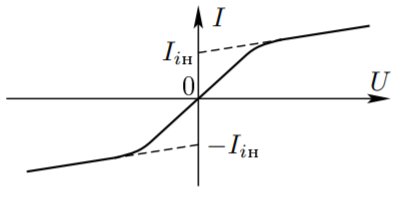
\includegraphics[scale=0.8]{4.png}
	\end{wrapfigure}
	Зависимость выглядит примерно так.
	Из формулы можно найти формулу для $T_e$: для $U=0$ мы найдём $I_{i\text{н}}$, продифференцируем в точке $U=0$ и с учётом $\text{th}~\alpha \approx \alpha$ при малых $\alpha$ и $A\rightarrow 0$ получим:
	\begin{equation}
		kT_e = \dfrac{1}{2}\dfrac{eI_{i\text{н}}}{\dfrac{dI}{dU}|_{U=0}}.
	\end{equation}
	\section*{Описание установки}
	\begin{center}
		
\includegraphics[scale=0.9]{1.png}
	\end{center}
	Стеклянная газоразрядная трубка имеет холодный (ненакаливаемый) полый катод, три анода и \textit{геттерный} узел -- стеклянный баллон, на внутреннюю повехность которого напылена газопоглощающая плёнка (\textit{геттер}). Трубка наполнена изотопом неона $^22$Ne при давлении 2 мм рт. ст. Катод и один из анодом (I и II) с помощью переключателя $\Pi_1$ подключается через балластный резистор $R_\text{б}$ ($\approx 450$ кОм) к регулируемому ВИП с выкодным напряжением до 5 кВ.\\
	При подключении к ВИП анода-I между ним и катодом возникает газовый разряд. Ток разряда измеряется миллиамперметром $A_1$, а падение напряжения на разрядной трубке -- цифровым вольтметром $V_1$, подключённым к трубке черезе высокоомный (25 МОм) делитель напряжения с коэффициентом $(R_1+R_2)/R_2 = 10$.\\
	При подключении к ВИП анода-II разряд возникает в пространстве между катодом и анодом-II, где находятся двойной зонд, используемый для диагностики плазмы положительного столба. Зонды изготовлены из молибденовой проволоки диаметром $d = 0.2$ мм и имеют длину $l = 5.2$ мм. Они подключены к источнику питания GPS через потенциометр $R$. Переключатель $\Pi_2$ позволяет изменять полярность напряжения на зондах. Величина напряжения на зондах изменяеься с помощью дискретного переключателя <<$V$>> выходного напряжения источника питания и потенциометра $R$, а измеряется цифровым вольтметром $V_2$. Для измерения зондового тока используется мультиметр $A_2$.
	
\section*{Задание}
\section*{Вольт-амперная характеристика разряда}
1) Собираем схему согласно установке и получаем следующие напряжения зажигания: \\
$U_{\text{заж}}^1 = 2,3$ кВ \\
$U_{\text{заж}}^2 = 2,25$ кВ \\
$U_{\text{заж}}^3 = 2,21$ кВ

2) Снимем требуемую ВАХ по показаниям $U_1$ и $I_1$:

\begin{tabular}{|c|c|c|c|c|c|c|c|c|c|c|c|c|c|c|c|c|c|c|}
\hline
$U_1$, В & 353  & 345  & 337  & 299  & 266  & 235  & 209  & 185  & 158  & 148  & 138  & 137  & 123  & 101  & 88   & 73   & 61   & 37   \\ \hline
$I_1$, мА & 0.31 & 0.64 & 1.03 & 1.31 & 1.47 & 1.71 & 1.98 & 2.33 & 2.65 & 2.85 & 3.09 & 3.23 & 3.61 & 4.03 & 4.28 & 4.54 & 4.72 & 5.03 \\ \hline
\end{tabular}

3)-5) Производим замер ВАХ двойного зонда при $I_{\text{р}} = 5$ мА

\begin{minipage}{1\textwidth}
      \begin{tikzpicture}
        \begin{axis}[
          width= 0.7\textwidth,
          height=,
          xlabel={$U_{2},~\text{В}$},
          ylabel={$I_{2},~\text{мкА}$},
          MyStyle1,
          ]
          \draw[black, domain=-30:30] plot (\x,9*\x);
          \draw[black, domain=-30:30] plot (\x,0.6*\x+82);
          \draw[black, domain=-30:30] plot (\x,1*\x-84);
          \addplot[purple, only marks] plot [error bars/.cd,
                x dir=both, x fixed = 0.05,
                y dir=both, y explicit,
                      ] table [
                      x=U, y=I, col sep=comma] {csv/3-5.csv};
          \addplot[purple, only marks] plot [error bars/.cd,
                x dir=both, x fixed = 0.05,
                y dir=both, y explicit,
                      ] table [
                      x=U_, y=I_, col sep=comma] {csv/3-5.csv};
        \end{axis}
      \end{tikzpicture}
\end{minipage}
Данные для построения ВАХа: \\
\begin{tabular}{|c|c|c|c|c|c|c|c|c|c|c|c|c|c|}
\hline
$U_2^+$, В   & 24.9  & 22.8  & 19.4  & 16.4  & 13.5 & 10.4 & 8.4  & 6.6  & 5.1  & 3.3   & 1.6   & 0.0   & 0.0   \\ \hline
$I_2^+$, мкА  & 110.6 & 109.3 & 106.1 & 101.2 & 93.6 & 81.4 & 71.5 & 62.1 & 53.2 & 41.4  & 28.4  & 14.0  & 0.0  \\ \hline
$U_2^-$, В & 0.0   & 1.4   & 2.9   & 3.9   & 5.4  & 7.4  & 9.1  & 11.2 & 14.4 & 17.4  & 20.3  & 22.4  & 24.9  \\ \hline
$I_2^-$, мкА & 10.0  & 21.7  & 33.7  & 41.1  & 51.8 & 63.6 & 73.1 & 84.2 & 97.6 & 106.6 & 112.5 & 115.3 & 117.7 \\ \hline
\end{tabular} \\
Для построения верного ВАХа смещаем положительные токи на 14.0 мкА, отрицательные на 10.0 мкА в сторону оси O$I$
\newpage
6) Производим замер ВАХ двойного зонда при $I_{\text{р}} = 2.96$ мА

\begin{minipage}{1\textwidth}
      \begin{tikzpicture}
        \begin{axis}[
          width= 0.7\textwidth,
          height=,
          xlabel={$U_{2},~\text{В}$},
          ylabel={$I_{2},~\text{мкА}$},
          MyStyle1,
          ]
          \draw[black, domain=-30:30] plot (\x,5*\x);
          \draw[black, domain=-30:30] plot (\x,0.55*\x+40);
          \draw[black, domain=-30:30] plot (\x,0.5*\x-45.5);
          \addplot[purple, only marks] plot [error bars/.cd,
                x dir=both, x fixed = 0.05,
                y dir=both, y explicit,
                      ] table [
                      x=U, y=I, col sep=comma] {csv/2.96.csv};
          \addplot[purple, only marks] plot [error bars/.cd,
                x dir=both, x fixed = 0.05,
                y dir=both, y explicit,
                      ] table [
                      x=U_, y=I_, col sep=comma] {csv/2.96.csv};
        \end{axis}
      \end{tikzpicture}
\end{minipage} \\
Данные для построения ВАХа: \\
\begin{tabular}{|c|c|c|c|c|c|c|c|c|c|c|c|c|c|}
\hline
$U_2^+$, В      & 24.9 & 22.3  & 19.8  & 16.3  & 13.7  & 10.9  & 8.2   & 6.4   & 4.5   & 2.9   & 1.1   & 0.0   & 0.0   \\ \hline
$I_2^+$, мкА    & 57.3 & 55.9  & 54.5  & 52.0  & 49.1  & 44.2  & 37.7  & 32.3  & 25.4  & 18.8  & 9.5   & 4.0   & 0.0   \\ \hline
$U_2^-$, В  & -0.0 & -1.5  & -3.0  & -4.6  & -5.7  & -7.5  & -9.5  & -11.4 & -13.9 & -17.0 & -19.6 & -22.2 & -24.9 \\ \hline
$I_2^-$, мкА  & -2.6 & -10.1 & -17.5 & -24.5 & -29.1 & -35.5 & -41.6 & -46.4 & -51.3 & -55.3 & -57.4 & -59.1 & -60.5 \\ \hline
\end{tabular}\\
Для построения верного ВАХа смещаем положительные токи на 4.0 мкА, отрицательные на 2.6 мкА в сторону оси O$I$ \\

Производим замер ВАХ двойного зонда при $I_{\text{р}} = 1.50$ мА

\begin{minipage}{1\textwidth}
      \begin{tikzpicture}
        \begin{axis}[
          width= 0.7\textwidth,
          height=,
          xlabel={$U_{2},~\text{В}$},
          ylabel={$I_{2},~\text{мкА}$},
          MyStyle1,
          ]
          \draw[black, domain=-30:30] plot (\x,4*\x);
          \draw[black, domain=-30:30] plot (\x,0.25*\x+20.5);
          \draw[black, domain=-30:30] plot (\x,0.3*\x-20.5);
          \addplot[purple, only marks] plot [error bars/.cd,
                x dir=both, x fixed = 0.05,
                y dir=both, y explicit,
                      ] table [
                      x=U, y=I, col sep=comma] {csv/1.5.csv};
          \addplot[purple, only marks] plot [error bars/.cd,
                x dir=both, x fixed = 0.05,
                y dir=both, y explicit,
                      ] table [
                      x=U_, y=I_, col sep=comma] {csv/1.5.csv};
        \end{axis}
      \end{tikzpicture}
\end{minipage} \newpage
Данные для построения ВАХа: \\
\begin{tabular}{|c|c|c|c|c|c|c|c|c|c|c|c|c|c|c|}
\hline
$U_2^+$, В    & 24.8 & 22.3 & 19.7 & 17.1 & 15.3 & 12.6 & 10.4 & 8.1  & 6.8  & 5.0  & 3.5  & 2.2  & 0.8  & 0   \\ \hline
$I_2^+$, мкА  & 26.5 & 25.8 & 25.0 & 24.2 & 23.6 & 22.4 & 20.8 & 18.4 & 16.5 & 13.4 & 9.9  & 6.7  & 2.9  & 0   \\ \hline
$U_2^-$, В & 0    & 1.6  & 3    & 4.7  & 6.5  & 8.8  & 10.5 & 13.0 & 15.1 & 18.0 & 20.3 & 22.2 & 24.9 & 0   \\ \hline
$I_2^-$, мкА   & 0.3  & 4.7  & 8.5  & 12.7 & 16.4 & 20   & 22   & 24.0 & 25.0 & 26.0 & 26.7 & 27.4 & 28.2 & 0.3 \\ \hline
\end{tabular}\\
Для построения верного ВАХа смещаем положительные токи на 4.0 мкА, отрицательные на 2.6 мкА в сторону оси O$I$

8) Строим ВАХ $U_{p}(I_p)$ по данным из 2) пункта:\\
\begin{minipage}{1\textwidth}
      \begin{tikzpicture}
        \begin{axis}[
          width= 0.7\textwidth,
          height=,
          xlabel={$U_{\text{р}},~\text{В}$},
          ylabel={$I_{\text{р}},~\text{мА}$},
          MyStyle1,
          ]
          \draw[red, domain=0:400] plot (\x,-0.0046666*\x+2.7);
          \addplot[purple, only marks] plot [error bars/.cd,
                x dir=both, x fixed = 0.05,
                y dir=both, y explicit,
                      ] table [
                      x=U, y=I, col sep=comma] {csv/2.csv};
          \addlegendentry{ВАХ разряда};
        \end{axis}
      \end{tikzpicture}
    \end{minipage}
По графику видно что максимальное дифференциальное сопротивление достигается на участке 250-350 В и оно равно: $R_{\text{диф}} = \frac{dU}{dI} = 215$ кОМ \\
Данный ВАХ близко соответствует ВАХу на участке Г-Д. \\
9) Строим все зондовые характеристики на одном графике теперь: \\
\begin{minipage}{1\textwidth}
      \begin{tikzpicture}
        \begin{axis}[
          width= 0.7\textwidth,
          height=,
          xlabel={$U_{2},~\text{В}$},
          ylabel={$I_{2},~\text{мкА}$},
          MyStyle1,
          ]
          \addplot[purple,mark=square*, only marks] plot [error bars/.cd,
                x dir=both, x fixed = 0.05,
                y dir=both, y explicit,
                      ] table [
                      x=U, y=I, col sep=comma] {csv/3-5.csv};
          \addplot[purple,mark=square*, only marks] plot [error bars/.cd,
                x dir=both, x fixed = 0.05,
                y dir=both, y explicit,
                      ] table [
                      x=U_, y=I_, col sep=comma] {csv/3-5.csv};
          \addplot[purple,mark=triangle*, only marks] plot [error bars/.cd,
                x dir=both, x fixed = 0.05,
                y dir=both, y explicit,
                      ] table [
                      x=U, y=I, col sep=comma] {csv/2.96.csv};
          \addplot[purple,mark=triangle*, only marks] plot [error bars/.cd,
                x dir=both, x fixed = 0.05,
                y dir=both, y explicit,
                      ] table [
                      x=U_, y=I_, col sep=comma] {csv/2.96.csv};
          \addplot[purple, only marks] plot [error bars/.cd,
                x dir=both, x fixed = 0.05,
                y dir=both, y explicit,
                      ] table [
                      x=U, y=I, col sep=comma] {csv/1.5.csv};
          \addplot[purple, only marks] plot [error bars/.cd,
                x dir=both, x fixed = 0.05,
                y dir=both, y explicit,
                      ] table [
                      x=U_, y=I_, col sep=comma] {csv/1.5.csv};
        \end{axis}
      \end{tikzpicture}
\end{minipage}\\
10) Также мы находим величины $\frac{dI}{dU}|_{U\rightarrow0}$ и $I_{i\text{н}}$ для всех исследуемых токов. \\
\begin{tabular}{|c|c|c|c|c|c|}
\hline
$N$ & $I$, мкА    & $\frac{dI}{dU}|_{U\rightarrow0}$, $\frac{\text{мкА}}{\text{В}}$  & $I_{i\text{н}}^+$, мкА& $I_{i\text{н}}^-$, мкА & $I_{i\text{н}}$, мкА \\ \hline
1 & 5.00 & $(9\pm0.5)$ & 82     & 84     & $(83\pm2)$   \\ \hline
2 & 2.96 & $(5\pm0.3)$ & 40     & 45.5   & $(43\pm3)$   \\ \hline
3 & 1.50 & $(4\pm0.3)$ & 21     & 20     & $(21\pm1)$   \\ \hline
\end{tabular} \\
11) - 13) Для нашей установки: $l = 5.2$ мм, $d= 0.2$ мм $\Rightarrow S \approx \pi d l = 3.27$ мм$^2$. По нашим формулам:
\begin{equation*}
    kT_e = \dfrac{1}{2}\dfrac{eI_{i\text{н}}}{\dfrac{dI}{dU}|_{U=0}},
\end{equation*}
\begin{equation*}
    I_{i\text{н}} = 0.4neS \sqrt{\frac{2kT_e}{m_i}} \Rightarrow n = \frac{I_{i\text{н}}}{0.4eS \sqrt{\frac{2kT_e}{m_i}}} \approx n_{i\text{н}} \approx n_e,
\end{equation*}
\begin{equation*}
    \omega_p = \sqrt{\frac{4\pi n_e e^}{m_e}},
\end{equation*}
\begin{equation*}
    r_{De} = \sqrt{\frac{kT_e}{4\pi n_e e^2}},
\end{equation*}
\begin{equation*}
    N_D = \frac{4\pi}{3} r^3_D n_i.
\end{equation*}
Так как $P \approx 2$ торр, $n = \frac{P}{kT_i} = 6.44\cdot 10^{22}$
\begin{equation*}
    \alpha = \frac{n_i}{n},
\end{equation*}
где $m_i = 22\cdot1.66\cdot10^{-27}$ кг.
\begin{equation*}
    \Delta(kT_e) = (k T_e) \cdot \left(\frac{\Delta I_{e\text{н}}}{I_{i\text{н}}} + \frac{\Delta(\frac{dI}{dU})|_{U=0}}{\frac{dI}{dU}|_{U=0}}\right),
\end{equation*}
\begin{equation*}
    \Delta n = n \cdot \left( \frac{\Delta(I_{i\text{н}})}{I_{i\text{н}}} + \frac{1}{2} \frac{\Delta (kT_e)}{kT_e}\right),
\end{equation*}
\begin{equation*}
    \Delta \omega_p = \left( \frac{\Delta n_e}{n_e}\right)
\end{equation*}
\begin{equation*}
    \Delta r_{De}/_{D} = r_{De} \left( \frac{\Delta (kT_e)}{kT_e} + \frac{\Delta n_e}{n_e}\right) 
\end{equation*}

Основной вклад в погрешности идет от несовпадения значений $\frac{dI}{dU}|_{U=0}$ и $I_{i\text{н}}$ при различных проведениях касательных. Погрешности будут указаны сразу в таблицах. \\
\begin{tabular}{|c|c|c|c|}
\hline
$N$     & 1    & 2    & 3    \\ \hline
$I_i$, мкА    & 5.00 & 2.96 & 1.50 \\ \hline
$kT_e$, эВ    & $4.6\pm0.4$  & $4.3\pm0.3$  & $2.6\pm0.3$  \\ \hline
$n_e$, $10^{16}$ м$^{-3}$     & $2.3\pm0.3$ & $4.5\pm0.3$ & $7.8\pm0.4$ \\ \hline
$\omega_p$, $10^9 \frac{\text{рад}}{\text{с}}$     & $8.3\pm0.5$ & $11.4\pm0.6$ & $15.3\pm0.8$ \\ \hline
$r_{De}$, мкм & $92\pm9$  & $65\pm6$ & $60\pm6$ \\ \hline
$r_D$, мкм  & $7.9\pm0.8$  & $5.3\pm0.5$  & $4.2\pm0.4$  \\ \hline
$N_D$  & $48\pm6$ & $35\pm5$ & $25\pm4$ \\ \hline
$\alpha \cdot 10^{-7}$     & $3.3\pm0.6$  & $7.4\pm0.9$  & $13\pm1$ \\ \hline
\end{tabular} \\
{\large\textbf{Вывод:}} мы происследовали ВАХ разряда, который совпал с куском зависимости Г-Д. Также получили значения в среднем с точностью 10\% значения которых близки к табличным и отличаются от них не более чем на 20\%.  

\end{document}